\documentclass[../main.tex]{subfiles}
 
\begin{document}

In English, this research concerns the problem of conducting surveillance in a designated, square-shaped area consisting of $d\times d$ unit squares. Enemy sensors are placed throughout this area; every sensor has the same sensing radius $r$. The set $L$ contains the coordinate location for each sensor. We have a specific number $n$ of \acp{uav} on hand; every \ac{uav} has the same battery capacity $b$.

The goal is to fly the \acp{uav} through the designated area so as to maximize surveillance capabilities. Each \ac{uav} starts and ends its flight outside the designated area (start and finish do not have to be in the same location). The \ac{uav} depletes one unit of battery per unit square visited. The current constraints, of course, imply that a \ac{uav} cannot sit in a non-edge square with a remaining capacity of zero. Because each unit square can be uniquely observed exactly once, we wish to maximize the total number of unique squares visited by all \acp{uav}.

We also wish to minimize risk. Because the sensors each have a known sensing radius, up to one-hundred percent of each unit square can be watched by the surrounding sensors. If (say) thirty percent of a unit square is covered by some combination of sensors, then each \ac{uav} that passes through said square has a thirty percent chance of being detected. We wish to minimize the sum of each \ac{uav}'s average chance of detection.

Of course, the individual impact of coverage and risk values must be finely-tuned: if coverage is too important, the \acp{uav} will accept too much risk; if coverage is not important enough, the \acp{uav} will refuse to visit squares with any risk.

\figurename \ \ref{fig:problem-visual} displays a specific \probs instance. One can clearly see the constraints on the system and the desired outcome by referencing this figure. Because \probs is such a difficult problem, this simple problem instance already entails a vast search space \cite{Liu2018, Caska2016, Lamont2007}. Thus, our algorithmic techniques must filter out poor solutions and exploit patterns in the space to identify adequate solutions.

\begin{figure}
    \centerline{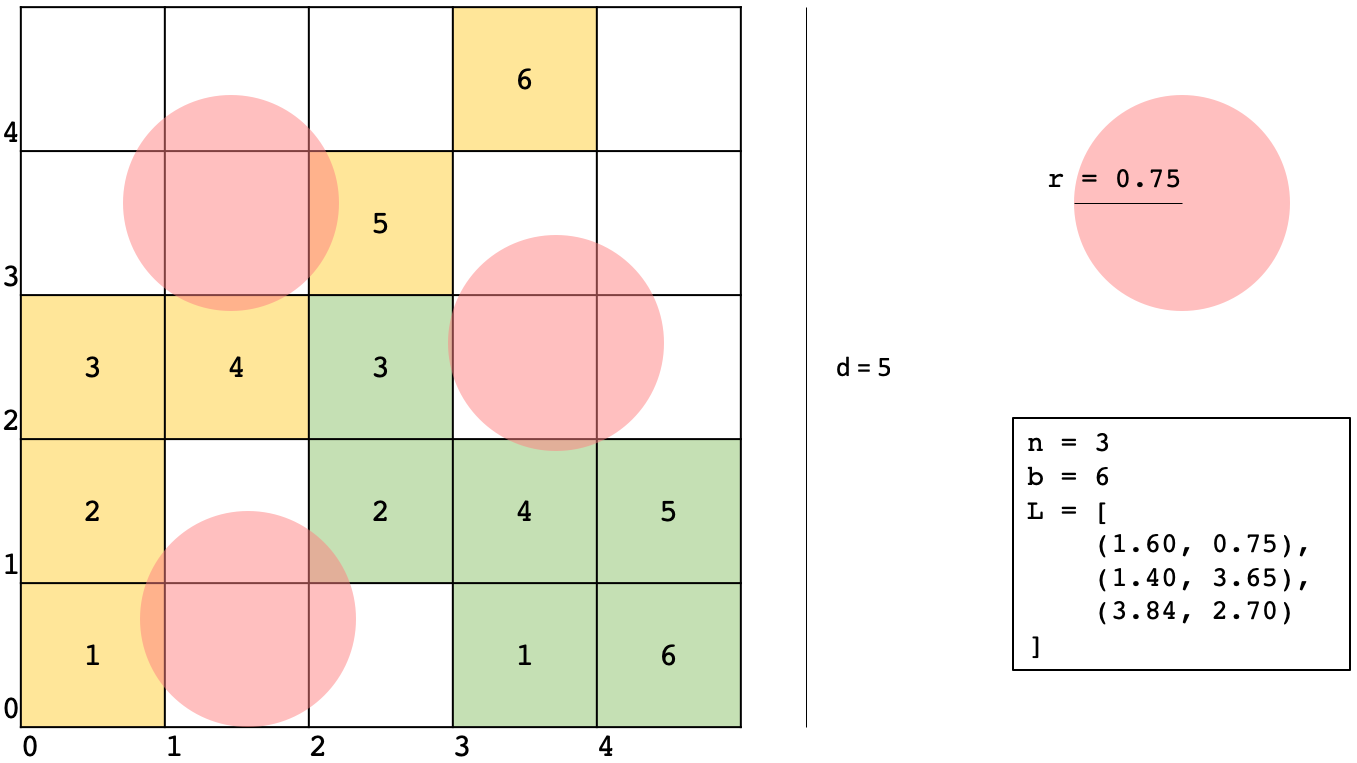
\includegraphics[width=\columnwidth]{problem-visual.png}}
    \caption{An example problem instance. The green and yellow squares depict the paths for two \acp{uav}. The red circles depict the coverage area for each of three \ac{uav} detectors.}
    \label{fig:problem-visual}
\end{figure}

Mathematically, the problem domain for \probs can be summarized as follows:

\begin{itemize}
    \item $D_i$, input domain

    \begin{itemize}
        \item $n$, the number of \acp{uav} available for scheduling
        \item $b$, the (integer) battery capacity of each \ac{uav}
        \item $L$, a list of all enemy sensor $(x,y)$ locations
        \item $r$, the sensing radius of the enemy sensors
        \item $d$, the (integer) side length of the surveillance area
    \end{itemize}
    
    \item Input conditions
    \begin{itemize}
        \item $\forall i\in \{n,b,|L|,r,d\}, i>0$; each of $n$, $b$, $|L|$, $r$, $d$ must be greater than $1$ to ensure the problem is nontrivial
        \item $\forall(x,y)\in L, 0\leq x<d, 0\leq y<d$; each sensor must be within the bounds of the surveillance area
    \end{itemize}
    
    \item $D_o$, output domain
    \begin{itemize}
        \item $P$, the set of \ac{uav} paths

        \item $V_P=0.90\times total\_ratio + 0.10\times edge\_ratio - 0.25\times (same\_repeats + other\_repeats) - 0.50\times risk$
        \begin{itemize}
            \item $total\_ratio=squares\_covered\div d^2$
            \item $edge\_ratio=edges\_covered\div (4d-4)$
            \item $same\_repeats$, number of times a \ac{uav} visits a square it has already visited
            \item $other\_repeats$, number of times a \ac{uav} visits a square another \ac{uav} has already visited
            \item $risk=total\_risk\div path\_length$
        \end{itemize}
    \end{itemize}
    
    \item Output conditions
    \begin{itemize}
        \item $|P|=n$; every \ac{uav} must have a path (even if the path is empty)
        \item $\forall p\in P, |p|\leq b$; no \ac{uav} can fly more than $b$ unit squares
        \item $\forall p\in P, \ edge(first(p)) = 1, \ edge(last(p)) = 1$; every \ac{uav} must start and end on an edge square
        \item $\forall Q, \ Q\neq P \Rightarrow V_Q<V_P$; the value of the path set $P$ must be maximal
    \end{itemize}

    \pagebreak

    \item Objective
    \begin{itemize}
        \item Maximize $V$, the overall state value
        \begin{itemize}
            \item Maximize $\sum_{i=1}^{n}{squares\_covered_i}$
            \item Minimize $\sum_{i=1}^{n}{risk_i}$
        \end{itemize}

        \item Employ deterministic, stochastic, and local algorithmic approaches to identify the best possible solution
        \item Conduct performance analyses of the approaches
    \end{itemize}
    
    \item Problem domain complexity
    \begin{itemize}
        \item \ac{mcp} is \ac{npc}
        \item \ac{mrp} is \ac{npc}
        \item See Appendix \ref{app:complexity} for more information (including \ac{npc} proofs and a discussion of the overall \probs complexity)
    \end{itemize}
\end{itemize}

\end{document}